%% bpmlr.tex
%% V0.1
%% 2015/01/01
%% by Mack Sweeney

\documentclass[10pt]{proc}


% *** CITATION PACKAGES ***
%
\usepackage{cite}
% cite.sty was written by Donald Arseneau
% V1.6 and later of IEEEtran pre-defines the format of the cite.sty package
% \cite{} output to follow that of IEEE. Loading the cite package will
% result in citation numbers being automatically sorted and properly
% "compressed/ranged". e.g., [1], [9], [2], [7], [5], [6] without using
% cite.sty will become [1], [2], [5]--[7], [9] using cite.sty. cite.sty's
% \cite will automatically add leading space, if needed. Use cite.sty's
% noadjust option (cite.sty V3.8 and later) if you want to turn this off.
% cite.sty is already installed on most LaTeX systems. Be sure and use
% version 4.0 (2003-05-27) and later if using hyperref.sty. cite.sty does
% not currently provide for hyperlinked citations.
% The latest version can be obtained at:
% http://www.ctan.org/tex-archive/macros/latex/contrib/cite/
% The documentation is contained in the cite.sty file itself.


% *** OTHER BIBLIOGRAPHY PACKAGES ***
%
%\usepackage[numbers]{natbib}


% *** GRAPHICS RELATED PACKAGES ***
%
\usepackage[pdftex]{graphicx}
% declare the path(s) where your graphic files are
\graphicspath{{./graphics/}}
% and their extensions so you won't have to specify these with
% every instance of \includegraphics
\DeclareGraphicsExtensions{.pdf,.jpeg,.png}

\usepackage{scalerel}
\usepackage{mdframed}

% For graphical models:
\usepackage{tikz}
\usetikzlibrary{bayesnet}


% *** MATH PACKAGES ***
%
\usepackage[cmex10, fleqn]{amsmath}
\usepackage{bm}
\usepackage{bbm}
\usepackage{amssymb}
\usepackage{mathtools}
\usepackage{etoolbox}
% A popular package from the American Mathematical Society that provides
% many useful and powerful commands for dealing with mathematics. If using
% it, be sure to load this package with the cmex10 option to ensure that
% only type 1 fonts will utilized at all point sizes. Without this option,
% it is possible that some math symbols, particularly those within
% footnotes, will be rendered in bitmap form which will result in a
% document that can not be IEEE Xplore compliant!
%
% Also, note that the amsmath package sets \interdisplaylinepenalty to 10000
% thus preventing page breaks from occurring within multiline equations. Use:
\interdisplaylinepenalty=2500
% after loading amsmath to restore such page breaks as IEEEtran.cls normally
% does. amsmath.sty is already installed on most LaTeX systems. The latest
% version and documentation can be obtained at:
% http://www.ctan.org/tex-archive/macros/latex/required/amslatex/math/


% *** SPECIALIZED LIST PACKAGES ***
%
\usepackage{algorithm}
\usepackage[noend]{algpseudocode}


% *** ALIGNMENT PACKAGES ***
%
\usepackage{array}
\usepackage{booktabs}
% Frank Mittelbach's and David Carlisle's array.sty patches and improves
% the standard LaTeX2e array and tabular environments to provide better
% appearance and additional user controls. As the default LaTeX2e table
% generation code is lacking to the point of almost being broken with
% respect to the quality of the end results, all users are strongly
% advised to use an enhanced (at the very least that provided by array.sty)
% set of table tools. array.sty is already installed on most systems. The
% latest version and documentation can be obtained at:
% http://www.ctan.org/tex-archive/macros/latex/required/tools/


% *** SUBFIGURE PACKAGES ***
%\usepackage[tight,footnotesize]{subfigure}
% subfigure.sty was written by Steven Douglas Cochran. This package makes it
% easy to put subfigures in your figures. e.g., "Figure 1a and 1b". For IEEE
% work, it is a good idea to load it with the tight package option to reduce
% the amount of white space around the subfigures. subfigure.sty is already
% installed on most LaTeX systems. The latest version and documentation can
% be obtained at:
% http://www.ctan.org/tex-archive/obsolete/macros/latex/contrib/subfigure/
% subfigure.sty has been superceeded by subfig.sty.

%\usepackage[caption=false]{caption}
%\usepackage[font=footnotesize]{subfig}
% subfig.sty, also written by Steven Douglas Cochran, is the modern
% replacement for subfigure.sty. However, subfig.sty requires and
% automatically loads Axel Sommerfeldt's caption.sty which will override
% IEEEtran.cls handling of captions and this will result in nonIEEE style
% figure/table captions. To prevent this problem, be sure and preload
% caption.sty with its "caption=false" package option. This is will preserve
% IEEEtran.cls handing of captions. Version 1.3 (2005/06/28) and later 
% (recommended due to many improvements over 1.2) of subfig.sty supports
% the caption=false option directly:
\usepackage[caption=false,font=footnotesize]{subfig}



% *** FLOAT PACKAGES ***
%
\usepackage{fixltx2e}
% fixltx2e, the successor to the earlier fix2col.sty, was written by
% Frank Mittelbach and David Carlisle. This package corrects a few problems
% in the LaTeX2e kernel, the most notable of which is that in current
% LaTeX2e releases, the ordering of single and double column floats is not
% guaranteed to be preserved. Thus, an unpatched LaTeX2e can allow a
% single column figure to be placed prior to an earlier double column
% figure. The latest version and documentation can be found at:
% http://www.ctan.org/tex-archive/macros/latex/base/

\usepackage{stfloats}
% stfloats.sty was written by Sigitas Tolusis. This package gives LaTeX2e
% the ability to do double column floats at the bottom of the page as well
% as the top. (e.g., "\begin{figure*}[!b]" is not normally possible in
% LaTeX2e). It also provides a command:
%\fnbelowfloat
% to enable the placement of footnotes below bottom floats (the standard
% LaTeX2e kernel puts them above bottom floats). This is an invasive package
% which rewrites many portions of the LaTeX2e float routines. It may not work
% with other packages that modify the LaTeX2e float routines. The latest
% version and documentation can be obtained at:
% http://www.ctan.org/tex-archive/macros/latex/contrib/sttools/
% Documentation is contained in the stfloats.sty comments as well as in the
% presfull.pdf file. Do not use the stfloats baselinefloat ability as IEEE
% does not allow \baselineskip to stretch. Authors submitting work to the
% IEEE should note that IEEE rarely uses double column equations and
% that authors should try to avoid such use. Do not be tempted to use the
% cuted.sty or midfloat.sty packages (also by Sigitas Tolusis) as IEEE does
% not format its papers in such ways.


% *** PDF, URL AND HYPERLINK PACKAGES ***
%
\usepackage{url}
% url.sty was written by Donald Arseneau. It provides better support for
% handling and breaking URLs. url.sty is already installed on most LaTeX
% systems. The latest version can be obtained at:
% http://www.ctan.org/tex-archive/macros/latex/contrib/misc/
% Read the url.sty source comments for usage information. Basically,
% \url{my_url_here}.


% BEGIN PAPER CONTENT
%
\title{Probabilistic Personalized Multi-Linear Regression}
\author{
    Mack Sweeney, Carlotta Domeniconi, Kathryn Laskey, Huzefa Rangwala\\
        George Mason University
}
\date{\today}


% New commands to be used in this report.
\newcommand*{\Scale}[2][4]{\scalebox{#1}{$#2$}}%
\newcommand*{\Resize}[2]{\resizebox{#1}{!}{$#2$}}%
\newcommand{\norm}[1]{\left\lVert#1\right\rVert}
\newcommand{\pluseq}{\mathrel{+}=}
\newcommand{\mineq}{\mathrel{-}=}
\newcommand{\asteq}{\mathrel{*}=}
\newcommand{\elips}[1]{\ldots#1\allowbreak}
\newcommand{\bc}{,\allowbreak}

\AtBeginEnvironment{align}{\par\footnotesize}
\AfterEndEnvironment{align}{\normalsize}
\AtBeginEnvironment{align*}{\par\footnotesize}
\AfterEndEnvironment{align*}{\normalsize}

\newtheorem{lemma}{Lemma}
\newtheorem{proof}{Proof}


\begin{document}
\maketitle


\begin{abstract}

\end{abstract}


\section{Introduction}

The goal of this study is  study the importance of user, item, and instructor
features in the GMU transcript data. To that end, we will generalize the
Personalized Multi-Linear Regression (PMLR) paper of Elbadrawy et al., interpet
it probabilistically, and use the probabilistic interpretation to derive one or
more notions of feature importance. The game plan for the study is as follows:

\begin{enumerate}
    \item  Generalize PMLR to Individualized Profile Regression (IPR). This step
        will allow us to use this same model to cluster items and instructors as
        well as users. The PMLR model clusters users. IPR will cluster any one
        entity. We will be able to learn three different models to study the
        user, item, and instructor profiles.
    \item  Derive efficient learning procedures for IPR. We intend to derive an
        SGD procedure and attempt to derive a coordinate descent (CD) and/or
        stochastic CD (SCD) procedure.
    \item  Determine a Bayesian interpretation of the IPR model. We find that
        the Gaussian Mixture Regression (GMR) model can be adapted to suit our
        needs. In particular, if we use individualized mixing weights (IGRM) and
        add bias terms (b-IGMR), we can view this as a Probabilistic IPR (PIPR).
    \item  Derive and implement efficient EM procedures for a Gaussian Mixture
        Model (GMM) and an individualized GMM (IGMM). This will help us
        understand how to do the same for GMR.
    \item  Come up with a biased version of the IGMM model, which we will call
        b-IGMM. The techniques used to do this will carry over to formulating a
        biased version of IGMR.
    \item  Derive an EM procdure for b-IGMM and implement it.
    \item  Implement the GMR model. This includes model selection (choice of K)
        and deriving and implementing an efficient EM procedure.
    \item  Extend GMR to use individualized mixing weights (IGMR). Derive EM
        procedure and implement.
    \item  Extend IGRM to use bias terms (b-IGMR = PIPR). Derive EM procedure
        and implement.
    \item  For each new model, implement a synthetic data generation process
        that mirrors the model's generative process. Test each model on all
        applicable synthetic datasets and compare.
    \item  Formalize the notion of feature importance for all 6 IPR variants.
    \item  Real-world dataset application and interpretation -- GMU transcript
        data.
\end{enumerate}

We can also think of several future studies that could branch off the current
one:

\begin{enumerate}
    \item  Run these methods on available MOOC datasets and use them to
        characterize the features in those datasets. Compare and contrast to
        feature importance in a traditional university setting.
    \item  Extend PIPR with a Bayesian interpretation and derive variational
        methods for learning. Demonstrate improvements and limitations; discuss
        tradeoffs.
    \item  Incorporate the notion of temporal relationships by combining
        concepts from linear dynamical systems to this model. Work from ideas of
        linear dynamical systems. This extension should allow us to study
        evolving entity clusters in terms of changes in feature importance
        among subpopulations of students/courses/instructors.
    \item  Consider the multi-task learning problem of learning the PIPR model
        jointly on several different datasets. For instance, we might have
        several datasets with traditional university data and several from MOOC
        courses and we would like to learn a model on all of them jointly.
\end{enumerate}

\paragraph{Outline}
The remainder of this paper is organized as follows.
Section~\ref{models} lays out each of the six variations of IPR, starting from
the generalization of PMLR to IPR and moving from there to each successive
alteration that eventually yields PIPR. Section~\ref{learning} describes
learning procedures for each model. Section~\ref{interpretation} formulates
feature importance metrics for each model. Section~\ref{experiments}
describes the synthetic data generation processes and results of running and
comparing the methods on this data and the real-world GMU transcript data. After
exploring performance, section~\ref{analysis} discusses how to perform
interpretable analysis using IPR and PIPR. Finally, section~\ref{previous work}
gives account of previous work, and section~\ref{conclusions} closes with
discussion of the work and directions for future work.

\section{Models}\label{models}

\subsection{Gaussian Mixture Regression}

\begin{figure}[th!]
  \centering
  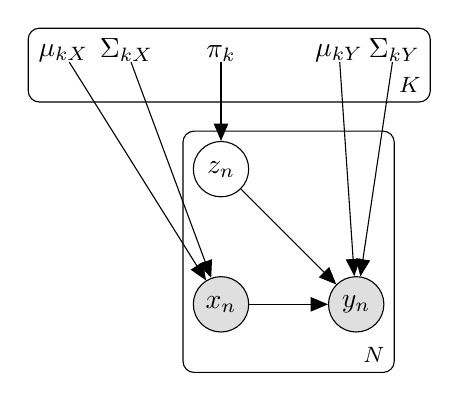
\begin{tikzpicture}

    % Define nodes
    \node[obs]                               (y) {$y_n$};
    \node[obs, left=of y]                    (x) {$x_n$};
    \node[latent, above=of x]                (z) {$z_n$};

    % y params
    \node[const, above=of z, xshift=1.5cm]  (my) {$\mu_{kY}$};
    \node[const, above=of z, xshift=2.2cm]   (sy) {$\Sigma_{kY}$};

    % x params
    \node[const, above=of z, xshift=-2.0cm]  (mx) {$\mu_{kX}$};
    \node[const, above=of z, xshift=-1.2cm]  (sx) {$\Sigma_{kX}$};

    % z params
    \node[const, above=of z]                 (pi) {$\pi_k$};

    % Connect the nodes
    \edge {x,z} {y};
    \edge {my,sy} {y};
    \edge {mx, sx} {x};
    \edge {pi} {z};

    % Plates
    \plate {data} {(y)(x)(z)} {$N$};
    \plate {models} {(my)(sy)(mx)(sx)(pi)} {$K$};

  \end{tikzpicture}
  \vspace{2pt}
  \caption{Bayesian PMLR Graphical Model} \label{fig:gmr-pgm}
\end{figure}

Below are the distributions that define the GMR model. First we have the joint
distribution:
%
\begin{align}
    f_{X,Y}(x,y) &= \sum_{k=1}^K
        \pi_k p(y|x; m_k(x), \sigma_k^2) p(x; \mu_{kX}, \Sigma_{kX}) \\
%%
    m_k(x) &= \mu_{kY} + \Sigma_{kYX} \Sigma_{kX}^{-1} (x - \mu_{kX})  \\
%%
    \sigma_k^2 &= \Sigma_{kYY} - \Sigma_{kYX} \Sigma_{kX}^{-1} \Sigma_{kXY}
%%
\end{align}

Marginal and conditional:
%
\begin{align}
    \nonumber
    f_X(x) &= \int f_{X,Y}(x,y) dy \\
           &= \sum_{k=1}^K \pi_k p(x; \mu_{kX}, \Sigma_{kX}) \\
%%
    f_{Y|X}(y|x) &= \sum_{k=1}^K w_k(x) p(y; m_k(x), \sigma_k^2) \\
%%
    w_k(x) &= \frac{ \pi_k p(x; \mu_{kX}, \Sigma_{kX}) }
                   { \sum_{j=1}^K \pi_j p(x; \mu_{jX}, \Sigma_{jX}) }
\end{align}

GMR(k) equations:
%
\begin{align}
    \nonumber
    m(x) &= E[Y|X = x] \\
         &= \sum_{k=1}^K w_k(x) m_k(x) \\
    \nonumber
    v(x) &= Var[Y|X = x] \\
         &= \sum_{k=1}^K w_k(x) (m_k(x)^2 + \sigma_k^2) - m(x)^2
\end{align}

\section{Learning}\label{learning}

\subsection{GMR}

Learning for the GMR model involves selecting the proper $K$ and then refining
the parameters for the $K$ chosen. This proceeds in 4 phases:
%
\begin{enumerate}
    \item  Construct kernel density estimate.
    \item  Combine pairwise ties and near-ties using the MoM.
    \item  Combine pairwise similar components using MoM or $\text{L}^2\text{E}$
        without data.
    \item  Combine pairwise similar components using $\text{L}^2\text{E}$ with
        data until there is only one component.
    \item  Using stats obtained during the previous phase, choose the best $K$.
        Then re-estimate parameters using $\text{L}^2\text{E}$ (if these were not
        already) stored.
\end{enumerate}

The steps listed above are as laid out by Scott and Szewczyk (2001). The
procedure was developed for univariate Gaussian Mixture Models. Sung adapts this
procedure for the multivariate case. There are several changes.
%
\begin{itemize}
    \item  First, he defines a custom Hellinger similarity metric for
        multivariate Gaussian PDFs.
    \item  Second, he uses Prim's algorithm to construct an MST of the
        components, which simplifies computation of similarity calculation from
        $O(N^2)$ to $O(Nlg(N))$.
    \item  Next, he uses only the MoM rather than the more computationally
        expensive $\text{L}^2\text{E}$ procedure.
    \item  Finally, after selecting the proper $K$, he uses an EM procedure for
        sharpening the fit obtained from MoM.
\end{itemize}

These changes require an EM procedure that can learn the GMR model parameters.
This seems to include the parameters for both $x_n$ and $y_n$. However, the EM
procedure presented in the appendix of Sung's thesis is for the normal
multivariate Gaussian Mixture Model rather than the one that includes paramters
for $y_n$.

\section{Interpretation}\label{interpretation}

\section{Experiments}\label{experiments}

\section{Analysis}\label{analysis}

\section{Previous work}\label{previous work}

\section{Conclusions}\label{conclusions}
We worked hard, and achieved very little.

% use section* for acknowledgement
\section*{Acknowledgment}
This research was funded by NSF IIS grant 1447489.


\bibliographystyle{siam}
\bibliography{refs}

\end{document}

